During our initial investigation, we identified a total of 2,058,408 road traffic incidents in the UK between 2005 and 2017.
Of these, 292,758 were categorised as severe accidents, accounting for 14\% of the overall incidents.
We began with 55 features to examine, and after refining the data by removing irrelevant factors and creating new ones, we were left with 219 features to analyse.

\subsubsection{Inferential Statistical Test}

We conducted a Chi-square test on each feature to assess which ones reject or fail to reject the null hypothesis ($H0$).
There are two methods to evaluate the null hypothesis using the Chi-square test: the test statistic method and the p-value method.
The test statistic method compares the calculated test statistic against a critical value from the Chi-square distribution table.
The p-value method compares the calculated p-value against a significance value, which we defined as $\alpha=0.05$.

Both methods were examined as an extra check since both should produce the same results.

Out of the 219 features, only 21 failed to reject $H0$ (See Fig. \ref{fig:null_hypothesis}).
Many features that rejected $H0$ had p-values near zero and a high Chi-square statistic (See Fig. \ref{fig:chi_squared_test}), indicating a significant relationship between the factor and accident severity.
As our objective was to find at least one factor that could reject $H0$, we can conclude that $H0$ is rejected, and the alternative hypothesis ($H1$) is accepted.

\begin{figure}[ht]
    \centering
    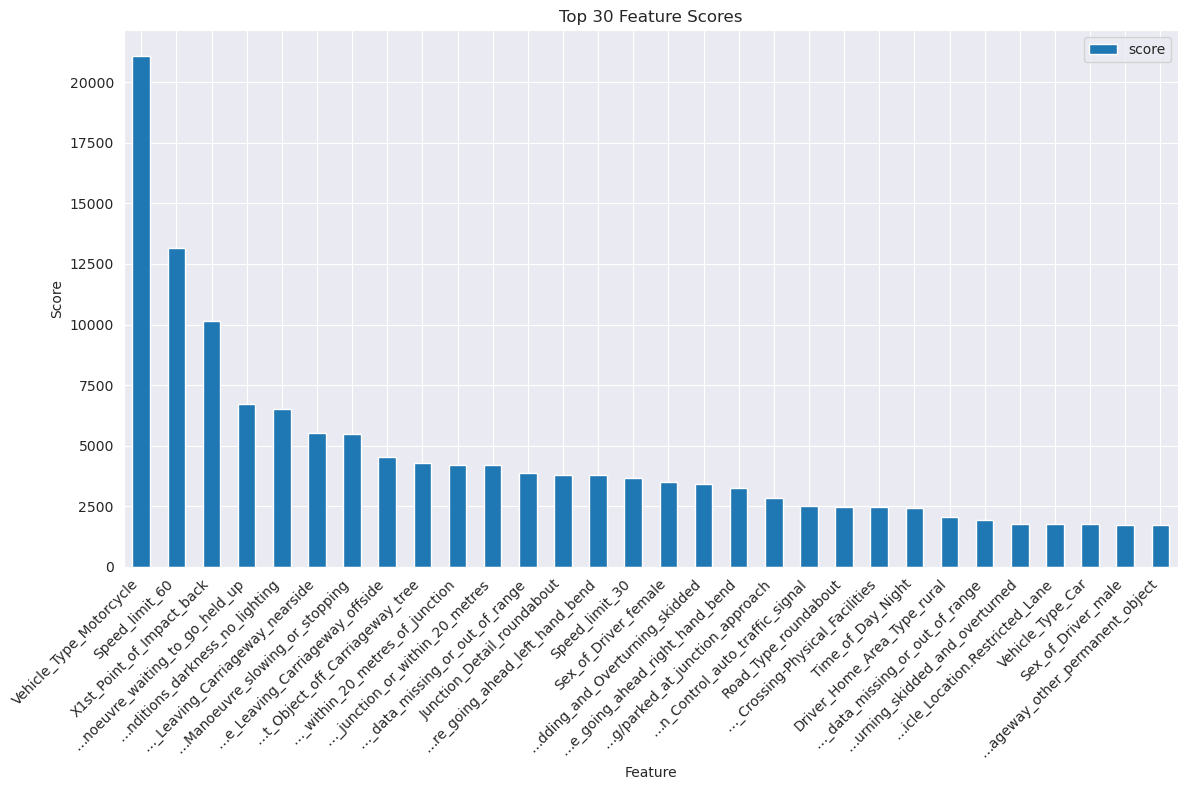
\includegraphics[width=0.5\textwidth]{images/ChiSquared_Feature_Scores}
    \caption{Chi-squared test using both categorical and numeric attributes.}
    \label{fig:chi_squared_test}
\end{figure}
\begin{figure}[ht]
    \centering
    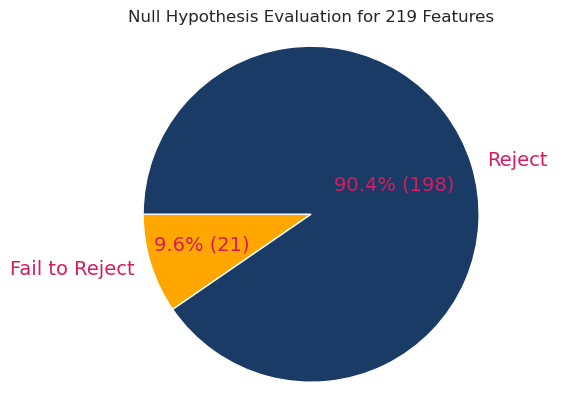
\includegraphics[width=0.5\textwidth]{images/Null_Hypothesis_Evaluation_pie}
    \caption{Chi-squared Test: Null Hypothesis $H0$ Evaluation.}
    \label{fig:null_hypothesis}
\end{figure}

From the 198 that reject $H0$, the following are the 10 showing the most significant relationship.

\begin{itemize}
    \item Vehicle Type: Motorcycle
    \item Speed Limit: 60 miles per hour
    \item 1st Point of Impact: Back
    \item Vehicle Manoeuvre
    \begin{itemize}
        \item Waiting to go, held up
        \item Slowing or stopping
    \end{itemize}
    \item Light Conditions:  Darkness, no lighting
    \item Vehicle Leaving Carriageway
    \begin{itemize}
        \item Nearside
        \item Offside
    \end{itemize}
    \item Hit Object off Carriageway: Tree
    \item Junction Location
    \begin{itemize}
        \item Not at or within 20 metres of junction
    \end{itemize}
\end{itemize}

However, only because a feature has a significant relationship with a severe accident, it does not imply causation such as traveling at 60 miles per hour will necessarily result in a hospital visit or death.
What the results indicate is the prevalence in a severe accident compared to less severe accidents.


Table \ref{tab:associations} presents the total number of incidents for each factor listed above, as well as the percentage contribution to the entire dataset and exclusively to severe incidents and Table \ref{tab:associations_reject} are the factors that fail to reject $H0$.

\begin{table}[ht]
    \centering
    \begin{tabular}{@{}lrrr@{}}
        \toprule
        & \multicolumn{1}{l}{Incidents} & \multicolumn{1}{l}{\% All} & \multicolumn{1}{l}{\% Severe} \\ \midrule
        Vehicle Type: Motorcycle & 173,110 & 8.41\% & 2.42\% \\
        Speed Limit: 60 & 317,097 & 15.41\% & 3.51\% \\
        1st Point of Impact: Back & 388,912 & 18.89\% & 1.41\% \\
        Waiting to Go / Held Up & 145,922 & 7.09\% & 0.38\% \\
        Slowing or Stopping & 171,469 & 8.33\% & 0.56\% \\
        Darkness, No Lighting & 99,708 & 4.84\% & 1.21\% \\
        Leaving Carriageway: Nearside & 123,874 & 6.02\% & 1.39\% \\
        Leaving Carriageway: Offside & 63,189 & 3.07\% & 0.78\% \\
        Hit Object off Carriageway: Tree & 27,633 & 1.34\% & 0.41\% \\
        Not at or within 20m of Junction & 808,108 & 39.26\% & 6.76\% \\ \bottomrule
    \end{tabular}
    \vspace{5}
    \caption{Significant associations with severe accidents}
    \label{tab:associations}
\end{table}

\begin{table}[ht]
    \centering
    \begin{tabular}{@{}lrrr@{}}
        \toprule
        & \multicolumn{1}{l}{Incidents} & \multicolumn{1}{l}{\% All} & \multicolumn{1}{l}{\% Severe} \\ \midrule
        Hit object: Bridge (roof) & 368 & 0.18\% & 0.03\% \\
        Speed limit 15 & 11 & 0.01\% & 0.00\% \\
        Defective road sign or marking & 3,197 & 15.53\% & 2.22\% \\
        Age band of driver 0--5 & 125 & 0.61\% & 0.09\% \\
        Special condition: Mud & 5,193 & 25.23\% & 3.63\% \\
        Commuting to/from work & 202,525 & 98.39\% & 14.03\% \\
        Left-hand drive vehicle & 3,887 & 18.88\% & 2.60\% \\
        Age band of driver 6--10 & 882 & 4.28\% & 0.66\% \\
        Carriageway hazard: Vehicle load & 2,852 & 13.86\% & 2.06\% \\
        Speed limit 10 & 13 & 0.06\% & 0.02\% \\
        Snowing with high winds & 2,635 & 12.80\% & 1.70\% \\
        Speed limit 40 & 187,000 & 90.85\% & 12.81\% \\
        Overtaking nearside & 10,658 & 51.78\% & 7.65\% \\
        Speed limit 70 & 183,791 & 89.29\% & 12.82\% \\
        Journey as part of work & 391,713 & 190.30\% & 26.89\% \\
        Raining with high winds & 27,813 & 13.51\% & 1.87\% \\
        Hit object: Road works & 889 & 4.32\% & 0.71\% \\ \bottomrule
    \end{tabular}
    \vspace{5}
    \caption{Features that fail to reject $H0$}
    \label{tab:associations_reject}
\end{table}

\subsubsection{Dimensionality Reduction}

We used the Recursive Feature Elimination method to determine the optimal number of features for predicting the severity of road traffic accidents using a machine learning model.
It starts with all available features and then iteratively removes one feature at a time by conducting a Chi-squared test to measure the strength of the relationship between each feature and the target variable.
The model's performance (recall score) on a test set is recorded and then continues with the iterative process until there are no more features to test.
The training/test split we used is 80\% to 20\% ratio.

By plotting the recall scores against the number of features, an \verb|elbow| point can be identified, which represents the ideal balance between the number of features and the model's performance.
In this case, the elbow point is at 43 features (See Fig. \ref{fig:recursive_feature_elimination}), suggesting that using these top 43 features is likely to yield the best prediction results for accident severity.

\begin{figure}[ht]
    \centering
    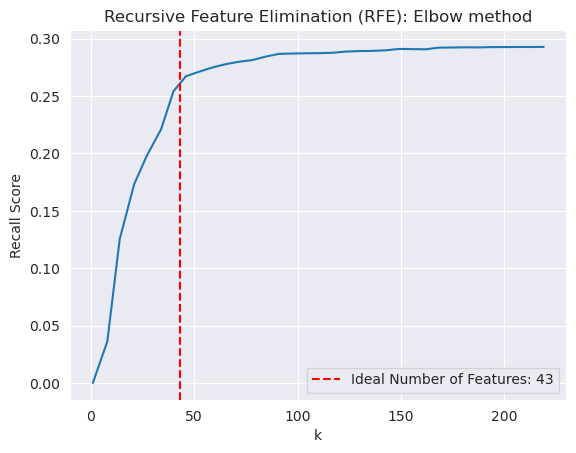
\includegraphics[width=0.5\textwidth]{images/Figure_Recursive Feature Elimination}
    \caption{Recursive Feature Elimination (RFE) Elbow Method}
    \label{fig:recursive_feature_elimination}
\end{figure}
